% Pour toute question sur l'utilisation de cette classe, écrivez à jerome.soucy(at)ulaval.ca
% Nécessite la classe Evaluation.sty dans le même dossier ou dans le PATH de votre système
% Nécessite le fichier logo_ul.pdf dans le même dossier un dans le PATH de votre système
\def\Ponderation{25}
\def\SigleNumero{STT-1920}
\def\NomCours{Méthodes statistiques}
\def\DateEvaluation{9 février 2022 de 13h30 à 15h20}
\def\Session{Hiver 2022}
\def\NomEvaluation{Examen 1}

% Ne rien mettre entre les accolades si l'enseignant (ou l'enseignante) est aussi le coordonnateur (ou la coordonnatrice)
\def\Coordonnatrice{}
\def\Coordonnateur{}

% Ne rien mettre entre les accolades s'il y a plus d'une section
\def\Enseignant{Julien Miron}
\def\Enseignante{}

% Ne rien mettre entre les accolades s'il s'agit d'un cours à section unique
% Mettre le nom de chacun des enseignants et enseignantes entre les accolades
% Une case à cocher sera générée pour chacune des sections

\def\SectionB{}
\def\SectionC{}
\def\SectionD{}

% Concerne seulement les travaux pratiques : écrire entre les accolades le nombre maximal de membres pour une équipe
\def\NombreLignes{}		

% Si vous souhaitez q'apparaisse une déclaration d'honneur au bas de la première page, écrivez quelque chose entre les accolades
\def\EnLigne{}

\def\Directives{
	\begin{enumerate}
			\item Matériel autorisé:
		\begin{itemize}
		    \item Calculatrice scientifique.
		    \end{itemize}
		\item Assurez-vous que cette \'evaluation comporte \numquestions ~questions réparties sur \numpages~pages, pour un total de \numpoints \ points.\
		\item \textbf{Veuillez ne pas débrocher votre examen.}
		\item Une table de la loi normale se trouve aux pages 12 et 14. Attention à ne rien débrocher.
		\item L'aide-mémoire est distribué séparément. \textbf{Assurez-vous d'en avoir reçu un!}
		\item Veuillez déposer votre carte d'identité \textbf{admise} avec photo sur votre bureau.\
		\item Vous devez donner les détails de vos démarches pour les questions 6 à 10.\
		\item Le verso des feuilles peut être utilisé comme brouillon, \textbf{mais ne sera pas corrigé}. Attention à ne rien débrocher.
	\end{enumerate}
}

% Veuillez indiquer le type d'évaluation entre crochets
% Examen : option à choisir pour un examen présentiel qui sera corrigé de manière classique. Un tableau des points sera affiché sur la page couverture.
% Gradescope : option à choisir pour un examen qui sera corrigé via Gradescope. Aucun tableau de pointage n'apparaîtra et il y a quelques différences au niveau de la mise en page
% TPS :
% TPF :
% Devoir :
\def\Gradescope{.} % Mode Gradescope activé (recto seulement). Mettre {} pour recto-verso.
\documentclass{Evaluation}
\begin{document}

%%%%%%%%%%%%%%%% QUESTION %%%%%%%%%%%%%%%%
	\begin{questions}
		\question[3] \begin{minipage}[b]{7cm}{
L'histogramme ci-contre représente la quantité de nourriture sèche ingérée en une journée  par 40 vaches choisies au hasard dans un élevage de 360 vaches. \\

On a les statistiques échantillonnales suivantes:\\

moyenne$= 18,8$ kg/jour\\

variance $= 23,6$ (kg/jour)$^2$

\vspace{1.5cm}
}
\end{minipage} \hspace{5mm}
%\begin{center}
\begin{minipage}[b]{9cm}{

\includegraphics[width=8.5cm]{Images/hist.png}}
%\end{center}
\end{minipage}

De quel type de variable s'agit-il? 
 

	
\begin{itemize}[label = { }]
		\item A) Quantitative discrète
		\item B) Quantitative continue
		\item C) Qualitative nominale
		\item D) Qualitative ordinale
	\end{itemize}




\begin{solution}
XXXXX
\end{solution}

%%%%%%%%%%%%%%%% QUESTION %%%%%%%%%%%%%%%%
\question[3] En utilisant l'histogramme de la question 1, dans quelle classe de l'histogramme se situe le quantile d'ordre 0,30?

	\begin{itemize}[label = {}]
		\item A) Dans la classe [10,15[
		\item B) Dans la classe [15,20[
		\item C) Dans la classe [20,25[
		\item D) Dans la classe [25,30[
		\item E) Dans la classe [30,35]
	\end{itemize}
 


\begin{solution}
XXXXXX
\end{solution}

\newpage
%%%%%%%%%%%%%%%% QUESTION %%%%%%%%%%%%%%%%
\question[3] Voici un diagramme qui représente la longueur des racines de 50 plants d'\textit{Amandinium gueralis} soumis à des stress lumineux. Les longueurs sont arrondies à l'unité.

%
\includegraphics[scale = 0.6]{boxplot1.pdf}

Lequel des énoncés suivants est faux concernant les données arrondies à l'unité?
	\begin{itemize}[label = {}]
		\item A) L'écart inter-quartile est de 2 cm.
		\item B) Le troisième quartile est égal à 4cm.
		\item C) Nous sommes certains qu'il y a au moins une plante dont la longueur des racines arrondie à l'unité est de 6 cm.
		\item D) La médiane et la moyenne sont nécessairement égales
	\end{itemize}
 

\begin{solution}

\end{solution}

%%%%%%%%%%%%%%%% QUESTION %%%%%%%%%%%%%%%%
\question[3] Deux futurs parents sont porteurs du génotype Aa, où «A» est l'allèle dominante et «a» est l'allèle récessive. À chaque grossesse, la probabilité de donner naissance à un enfant porteur de l'allèle dominante est de 75 \% et chacune des naissances est indépendantes des autres. Ce couple prévoit avoir 4 enfants. Soit les événements $W$:«Le deuxième enfant n'est pas porteur de l'allèle dominante» et $Y$:«Exactement trois des quatre enfants du couple sont porteurs de l'allèle dominante». Quelles sont les probabilités associées à ces deux événements?

\begin{itemize}[label = {}]
\item A) $P(W)=0,25$ et $P(Y)\approx 0,422$
\item B) $P(W)=0,25$ et $P(Y)\approx 0,047$
\item C) $P(W)=0,75$ et $P(Y)\approx 0,422$
\item D) $P(W)=0,75$ et $P(Y)\approx 0,047$
\end{itemize}

 


\begin{solution}
Réponse D)
\end{solution}


\question
\textbf{\textit{Pour les questions suivantes, inscrivez «Vrai» ou «Faux» dans les cases appropriées.}}

\begin{parts}
\part[2] Si X suit une loi normale
$\mathcal{N}(8, 25)$, nous avons: $P(X\leq 13)=P(Z\leq \frac{13-8}{5})=\Phi(\frac{13-8}{5})$, où $Z\sim\mathcal{N}(0,1)$.

 

\part[2] Deux événements A et B sont mutuellement exclusifs si et seulement si A et B sont indépendants.

 

\part[2] Si $R$ et $S$ sont deux événements indépendants, alors nous avons toujours $P(R\cup S)=P(R)P(S)$.

 

\part[2] Le coefficient binomial ${M \choose j}$ nous donne la probabilité de choisir $j$ éléments différents parmi $M$ éléments possibles.

 

\part[2] Si $X$ a une fonction de densité symétrique, alors nous sommes certains qu'il s'agit de la loi normale.

 

\part[2] Il est toujours possible d'identifier le minimum, la médiane et le maximum d'un échantillon sur un diagramme en boîte.

 

\part[2] On répète 12 fois de façon indépendante une épreuve de Bernoulli dont la probabilité de succès est de 0,80. Alors on peut dire que le nombre de succès suit une loi $\text{Binomiale}(n = 12, p = 0,8)$ et que le nombre d’échecs suit une loi $\text{Binomiale}(n = 12, p = 0,2)$.

 

\end{parts}

%%%%%%%%%%%%%%%% QUESTION %%%%%%%%%%%%%%%%
\question Le nombre de naissances quotidiennes dans un certain centre d’obstétrique suit une loi de Poisson de paramètre $\lambda=8$.
\medskip
\begin{parts}
\part[5] Quelle est la probabilité qu'il y ait 3 naissances ou plus dans ce centre lors d'un jour donné. Donnez les détails de votre démarche!

\vspace{13cm}
\end{parts}
Une infirmière inscrit chaque jour le nombre de naissances dans un fichier Excel, durant une année.
\begin{parts}
\setcounter{partno}{1}
\part[2] On s'attend à ce que la moyenne de ces 365 observations soit environ égale à quelle valeur?

\vspace{1cm}

\part[2] On s'attend à ce que la variance de ces 365 observations soit environ égale à quelle valeur?

\end{parts}

\newpage

%%%%%%%%%%%%%%%% QUESTION %%%%%%%%%%%%%%%%
\question\label{cable} Héma-Québec nous fournit les informations suivantes par rapport aux groupes sanguins:

\medskip

\begin{table}[h]
    \centering
\begin{tabular}{|c|c|}
\hline
    Groupe & Proportion\\
    \hline
     A&  0,43\\
     B& ?\\
     AB& 0,03 \\
     O& 0,46\\
     \hline
\end{tabular}
    \label{tab:my_label}
\end{table}

Notez que AB est un groupe en soi, ce n'est pas une combinaison des groupes A et B. De plus, un individu ne peut pas avoir plus d'un groupe sanguin et il n'y a aucun autre groupe que les quatre mentionnés dans le tableau.


\begin{parts}
\part[2] Le groupe sanguin est une variable aléatoire de quel type?
\vspace{1cm}
\part[6] Vous allez passer un test pour connaître votre groupe sanguin. Quelle est la probabilité que vous apparteniez au groupe B ou au groupe O ? Donnez les détails de votre démarche!

\vspace{8cm}
\end{parts}
Pour ce qui suit, on utilise la variable aléatoire $X$, qui prend la valeur $1$ si un individu appartient au groupe sanguin A et $0$, s'il appartient à un autre groupe, et la variable aléatoire Y, qui compte le nombre d'individus parmi 10 qui appartiennent au groupe sanguin A.
\begin{parts}
\setcounter{partno}{2}
\part[3] Quelle est la loi de $X$ ? Il est important de bien identifier le ou les paramètres.
\vspace{3cm}
\part[3] Quelle est la loi de $Y$ ? Il est important de bien identifier le ou les paramètres.
\end{parts}

\newpage
%%%%%%%%%%%%%%%% QUESTION %%%%%%%%%%%%%%%%
\question On suppose que la pression artérielle systolique (en mm Hg) suit une loi normale de moyenne 133 et de variance $6^2$. On utilisera $X$ pour dénoter cette variable aléatoire. Donc $X\sim\mathcal{N}(133, 6^2)$.

\begin{parts}
\part[3] Quelle est la probabilité qu'un individu choisi au hasard ait une pression artérielle systolique inférieure ou égale à 133? Justifiez votre réponse!

\vspace{3cm}

\part[8] Nous aimerions connaître la probabilité qu'un individu choisi au hasard ait une pression artérielle systolique inférieure à 124 ou supérieure à 139. Calculez cette probabilité en utilisant la table de la loi normale de la page précédente. Utilisez 4 chiffres après la virgule dans vos calculs et dans votre réponse. Donnez les détails de votre démarche!
\vspace{13cm}

\part[4] Si on prenait un échantillon de 100 personnes, quelle serait la variance de la moyenne échantillonnale $\Bar{X}$? Donnez la valeur de cette variance! Donnez les détails de votre démarche!

\end{parts}

\newpage

%%%%%%%%%%%%%%%% QUESTION %%%%%%%%%%%%%%%%
\question Une association agricole évalue qu'une brebis adulte coûte en moyenne 80\$ par année à nourrir, avec un écart-type de 12\$. Voici les diagrammes de la fonction de densité et de la fonction de répartition du modèle probabiliste supposé.

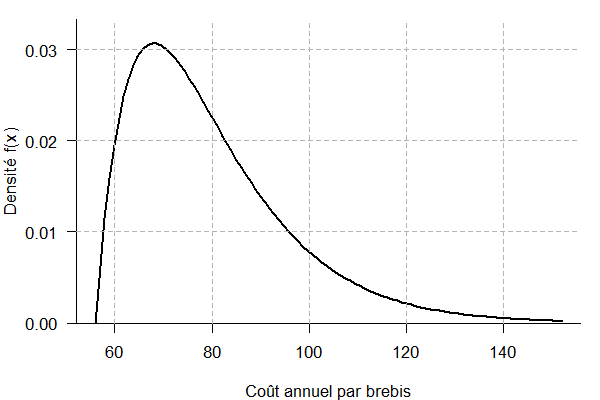
\includegraphics[width=8cm]{Images/chi-den.png}
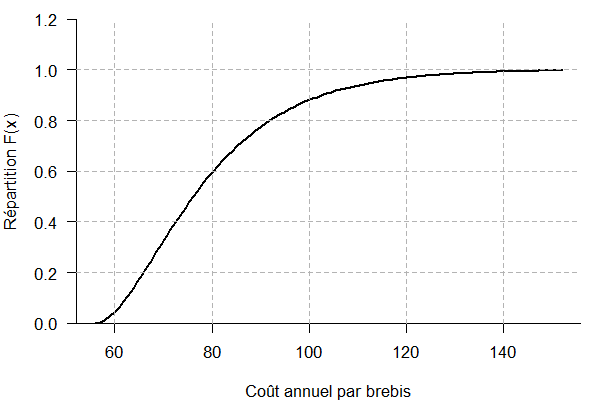
\includegraphics[width=8cm]{Images/chi-rep.png}

\begin{parts}
\part[2] En utilisant les diagrammes, quelle est la probabilité approximative que le coût annuel par brebis soit suppérieur à 80\$ ?

\vspace{2cm}

\part[2] En utilisant les diagrammes, dites si la loi normale convient pour modéliser cette variable aléatoire. Donnez au moins une raison!

\vspace{1.5cm}

\part[8] Une ferme possède un élevage de 400 brebis. Donnez une approximation de la probabilité que le montant annuel à débourser pour les nourrir dépasse 32120\$. Donnez les détails de votre démarche!

\end{parts}
\newpage


%%%%%%%%%%%%%%%% QUESTION %%%%%%%%%%%%%%%%

\question

Soit la variable aléatoire $X$ dont la fonction de densité est donnée par:

 \begin{equation*}
  f(x) = \begin{cases}
        2x, \text{ si } 0\leq x \leq 1\\
        0, \text{ sinon.}
        \end{cases}
 \end{equation*}
 
Nous avons les résultats suivants:

\begin{align*}
   \int_{0}^b2xdx&=b^2  & \int_{0}^1 2x^2dx&=\frac{2}{3}\\
\end{align*}
\begin{parts}
\part[2] Que vaut $P(X\leq 0.8)$? Donnez les détails de votre démarche!
\vspace{5cm}
\part[2] Que vaut $E(X)$ ? Donnez les détails de votre démarche!
\end{parts}
\end{questions}


\end{document} 
